%=======================================================================
\section{AMR Component} \label{s:component-amr}
%=======================================================================

The \code{Amr} component defines the data structures and data
structure parameters for the ``inter-resolution'' aspect of
distributed AMR hierarchies.  (The ``intra-resolution'' aspects are
defined using the \code{Array} component).  Both patch-based AMR, ala
\enzo, and octree-based AMR datastructures are supported.

Operations

The \code{Amr} component accesses the \code{Array} component to define
the ``intra-resolution'' aspect of field data on an AMR hierarchy, and
the
\code{Particles} component to define particles on the AMR

to, such as number of mesh
levels, grid patch properties, rebuild algorithm, dynamic load
balancing, refinement criteria, etc.

Hierarchy
Array


\begin{itemize}
\item hierarchy
\begin{item}
\item min\_levels 
\item max\_levels 
\end{item}
\item level
\item grid
\begin{itemize}
\item min\_size
\item max\_size
\item max\_aspect
\item quantum
\end{itemize}
\end{itemize}

\centerline{
\includegraphics[width=1.8in]{amr4-1.eps} \ \
            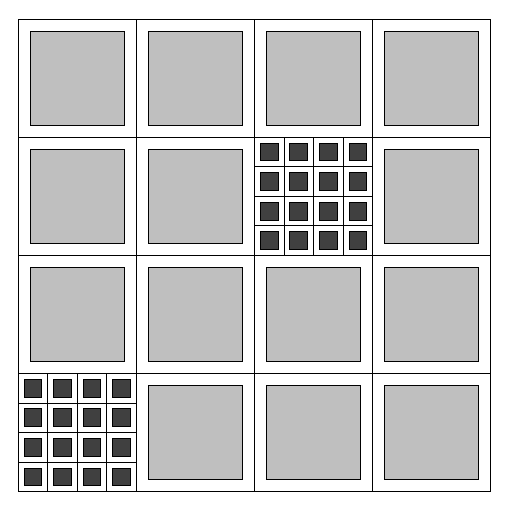
\includegraphics[width=1.8in]{amr4-2.eps} \ \
            \includegraphics[width=1.8in]{amr4-3.eps}}

\centerline{\includegraphics[width=1.8in]{amr2-1.eps} \ \
            \includegraphics[width=1.8in]{amr2-2.eps} \ \
            \includegraphics[width=1.8in]{amr2-3.eps}}
\ \\
\centerline{\includegraphics[width=1.8in]{amr2-4.eps} \ \
            \includegraphics[width=1.8in]{amr2-5.eps} \ \
            \includegraphics[width=1.8in]{amr2-7.eps}}
\ \\
\centerline{\includegraphics[width=1.8in]{amr2-8.eps} \ \
            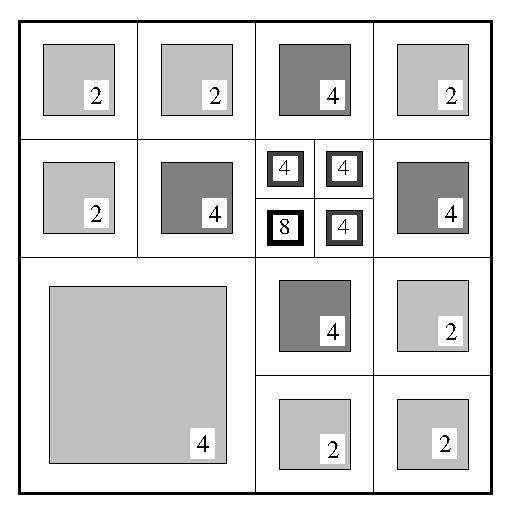
\includegraphics[width=1.8in]{amr2-9.eps} \ \
            \includegraphics[width=1.8in]{amr2-11.eps}}

%-----------------------------------------------------------------------
\subsection{Use Cases}
%-----------------------------------------------------------------------
%-----------------------------------------------------------------------
\subsection{Parameters}
%-----------------------------------------------------------------------
